
\documentclass[fleqn,addpoints]{exam}
\usepackage{amsmath}
\usepackage{graphicx}
\usepackage{float}
\usepackage{caption}

\printanswers

\ifprintanswers
\usepackage{2in1, lscape}
\fi

\title{Math 115 Chapter One Exam}
\date{December 7, 2010}

\author{}

\begin{document}

\maketitle

\ifprintanswers
\else
\vspace{0.2in}
\makebox[\textwidth]{Name:\enspace\hrulefill}
\vspace{0.2in}

\begin{center}
\gradetable[h][pages]
\bonusgradetable[h][pages]
\end{center}

\fi

% \section{Inequalities}

% In questions \ref{inequality:first}-\ref{inequality:last}, solve the inequalities.

% \begin{questions}
% \question[5] $\dfrac{x^2+3x-2}{x+4} > 0$
% \label{inequality:first}
% \begin{solution}[4 cm]
% \end{solution}

% \question[7] $\dfrac{2x+3}{x+2} > 2$
% \label{inequality:last}
% \begin{solution}[4 cm]
% \end{solution}

\section{Circles}

\begin{questions}

\question[5]
What is the equation of a circle with radius 5 and center $(-1, 2)$?
\begin{solution}[2 cm]
\[
  (x+1)^2 + (y-2)^2 = 5^2
\]

\end{solution}

\question
Using the equation: 
\[
  x^2 + 6x + y^2 - 4y = 3
\]

\label{circle}
\begin{parts}
\part[6] Put the equation standard form.
\begin{solution}[4 cm]
\begin{align*}
  x^2 + 6x + y^2 - 4y &= 3 \\
  x^2 + 6x +9 -9 + y^2 - 4y + 4 -4 &= 3 \\
  (x+3)^2 -9 + (y-2)^2 -4 &= 3 \\
  (x+3)^2 + (y-2)^2  &= 16 \\
  (x+3)^2 + (y-2)^2  &= 4^2 \\
\end{align*}

\end{solution}

\part[2] What is the center?
\begin{solution}[1 cm]
  $(-3, 2)$
\end{solution}

\part[2] What is the radius?
\begin{solution}[1 cm]
  4
\end{solution}

% \part[2] Draw the graph
% \begin{figure}[H]
%   \centering
%   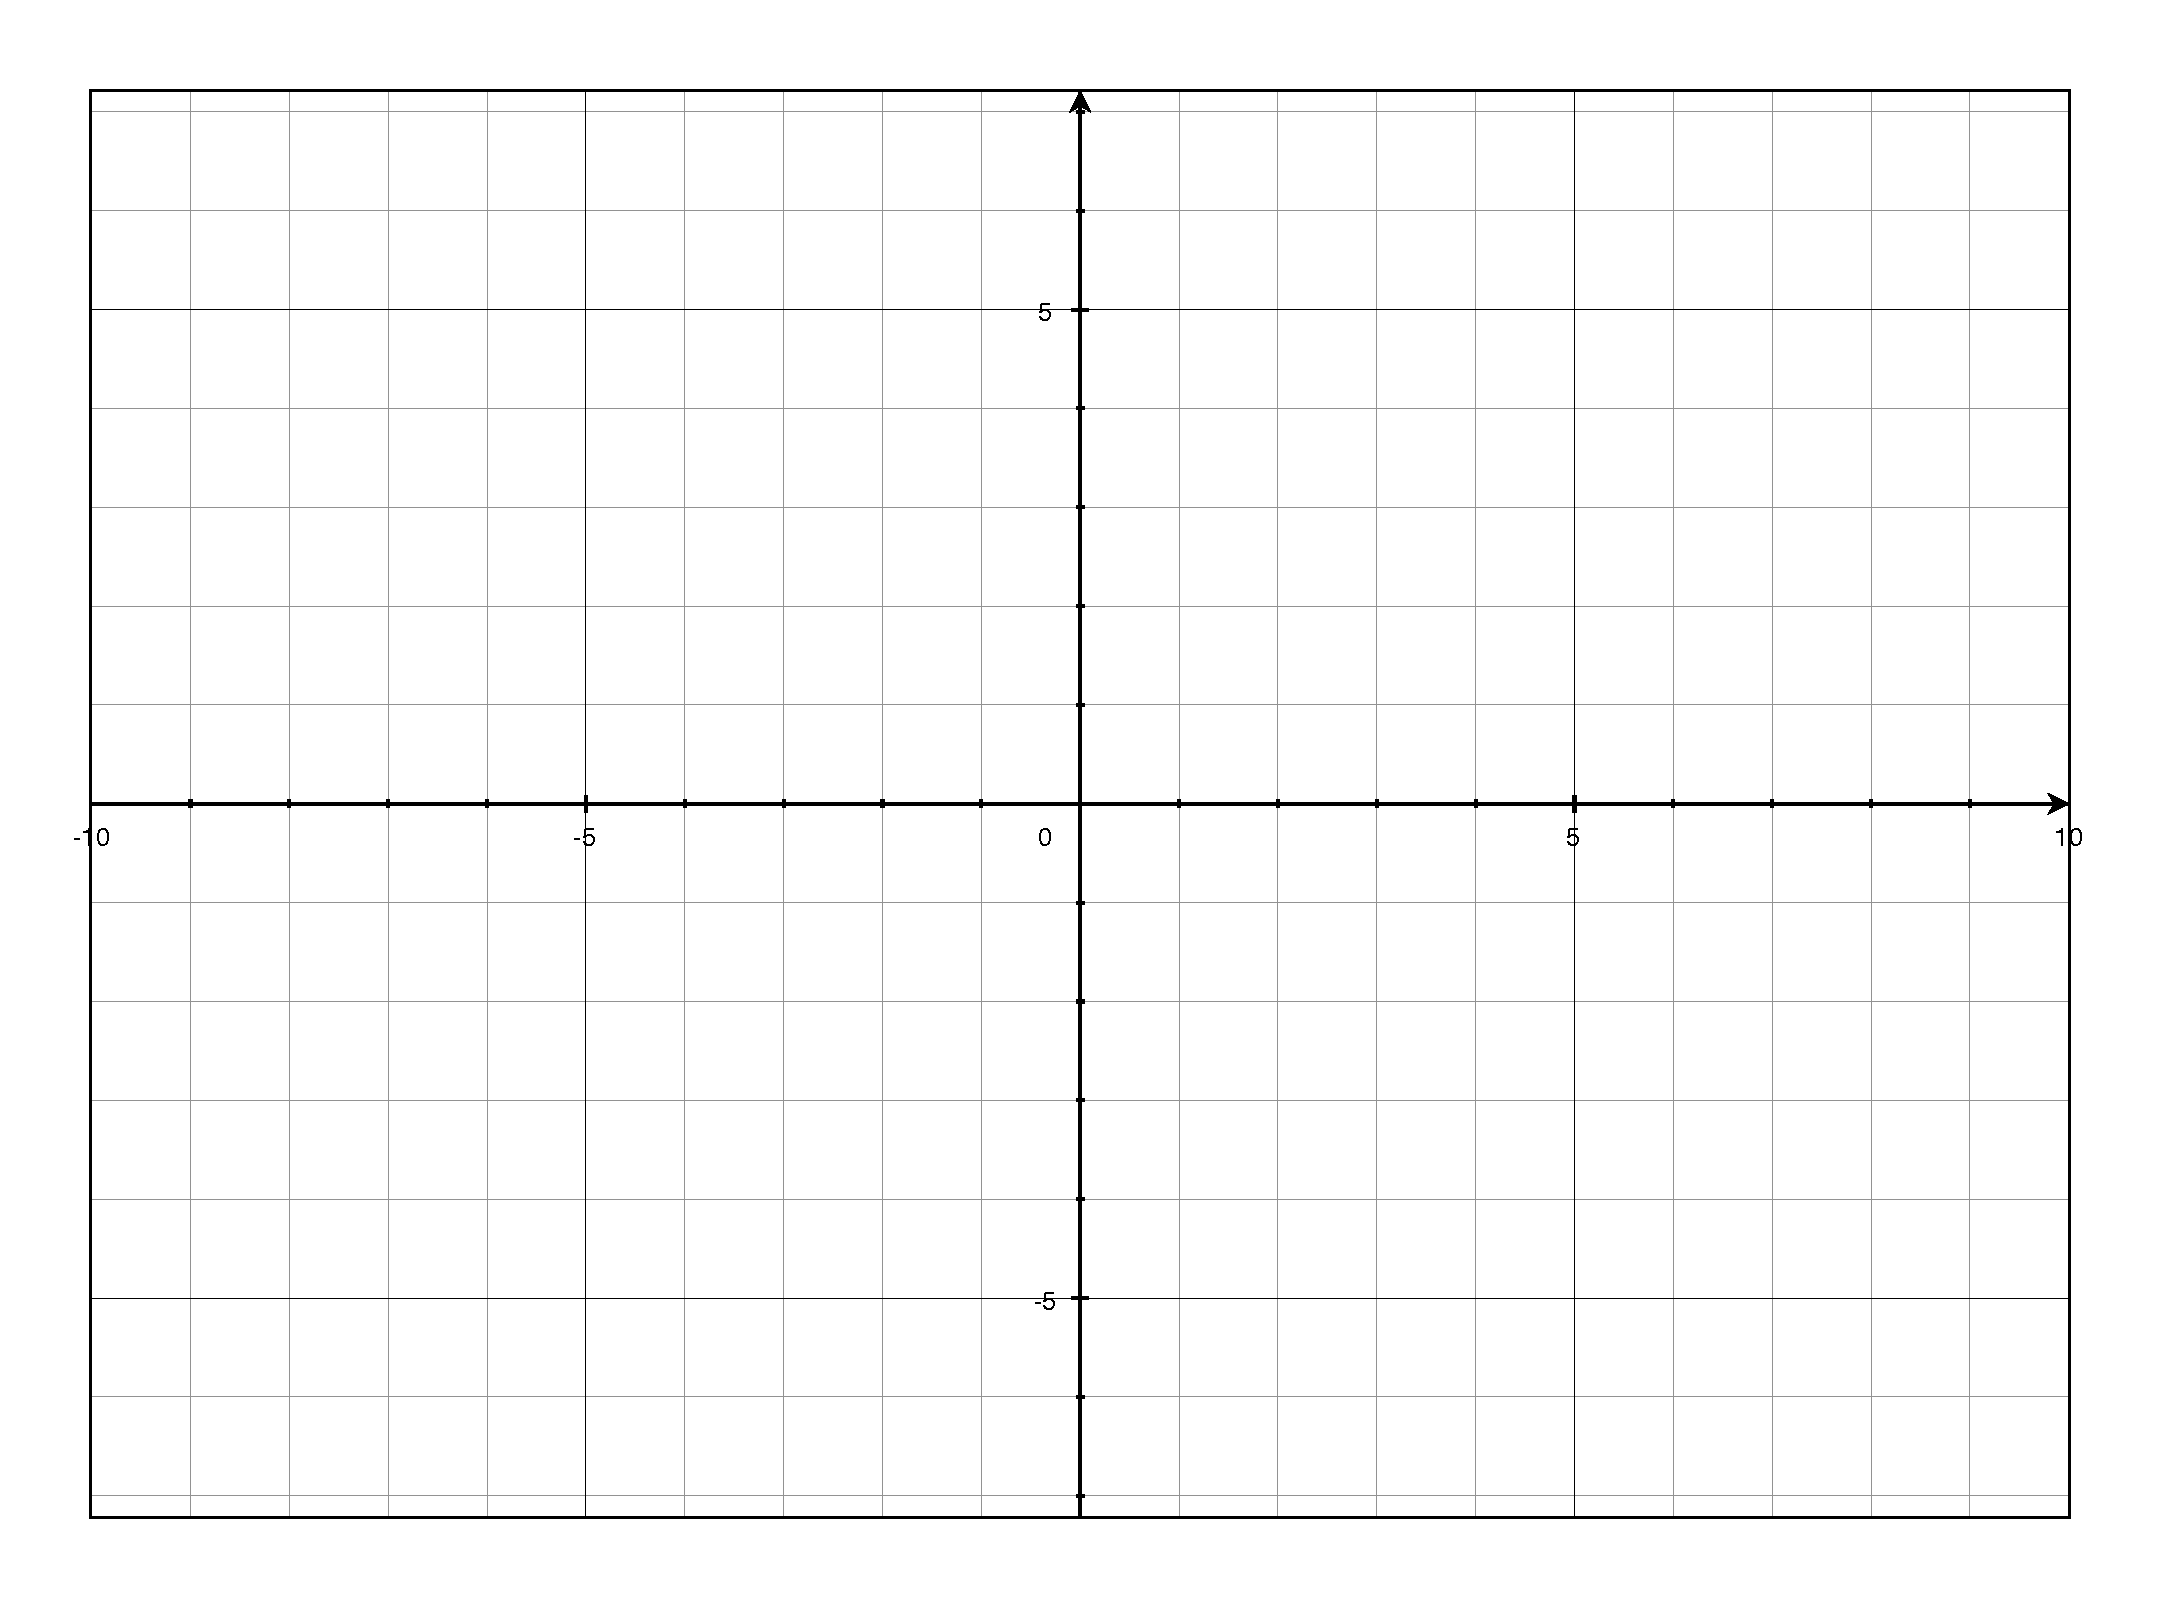
\includegraphics[width=14cm,height=10cm]{circle.eps}
%   \caption*{Problem \ref{circle}}
% \end{figure}

\end{parts}

\ifprintanswers
\else
\pagebreak
\fi

\section{Domain}

\question[5] 
Find the domain of: $f(x) = \sqrt{x^2-4}$
\begin{solution}[6 cm]
\begin{align*}
  x^2 - 4 &\geq 0 \\
  (x+2)(x-2) &\geq 0 \\
\end{align*}

\begin{tabular}{|c|c|c|c|c|c|}
\hline
  $x$     &  $< -2$ & $-2$ & $-2$ to $2$ & $2$ & $>2$ \\
\hline
\hline
  $x + 2$ &  $-$    & $0$  & $+$         & $+$ & $+$  \\
\hline
  $x-2$   &  $-$    & $-$  & $-$         & $0$ & $+$  \\
\hline
\hline
  $f(x)$  &  $+$    & 0    & $-$         & 0   & $+$  \\
\hline
\end{tabular}

From the last row, we can see that the domain is:  
\[
  (-\infty, -2] \cup [2, \infty)
\]
\end{solution}

\ifprintanswers
\pagebreak
\fi

\question[7] 
Find the domain of: $f(x) = \sqrt{\dfrac{x^2-x-2}{x+4}}$
\begin{solution}[5 cm]
\begin{align*}
  \frac{x^2-x-2}{x+4} &\geq 0 \\
  \frac{(x-2)(x+1)}{x+4} &\geq 0 \\
\end{align*}

\begin{tabular}{|c|c|c|c|c|c|c|c|}
\hline
  $x$     & $<-4$ & $-4$ & $-4$ to $-1$ & $-1$ & $-1$ to $2$ & $2$ & $>2$ \\
\hline
\hline
  $x + 4$ & $-$   & $0$    & $+$          & $+$ & $+$          & $+$ & $+$  \\
\hline
  $x + 1$ & $-$   & $-$    & $-$          & $0$ & $+$          & $+$ & $+$  \\
\hline
  $x - 2$ & $-$   & $-$    & $-$          & $-$ & $-$          & $0$ & $+$  \\
\hline
\hline
  $f(x)$  & $-$   & $\diamond$ & $+$          & $0$ & $-$          & $0$ & $+$  \\
\hline
\end{tabular}

From the last row, we can see that the domain is:
\[
  (-4, -1] \cup [2, \infty)
\]
\end{solution}

\ifprintanswers
\else
\pagebreak
\fi

\section{Combining Functions}

\question Let:
\begin{align*}
  f(x) &= 2x^2 + 1 \\
  g(x) &= 3x + 2
\end{align*}

\begin{parts}
\part[3] Find $(f+g)(x)$ and its domain
\begin{solution}[2 cm]
\[
  (f+g)(x) = 2x^2 + 3x + 3
\]

The domain is: $(-\infty, \infty)$

\end{solution}

% \part[3] Find $(f-g)(x)$ and its domain
% \begin{solution}[2.5 cm]
% \end{solution}

% \part[3] Find $(fg)(x)$ and its domain
% \begin{solution}[2.5 cm]
% \end{solution}

\ifprintanswers
\pagebreak
\fi

\part[3] Find $(f/g)(x)$ and its domain
\begin{solution}[2 cm]
\[
  (f/g)(x) = \frac{2x^2+1}{3x+2}
\]

The domain is: $x \neq -\frac{2}{3}$

\end{solution}

\part[3] Find $(f \circ g)(x)$ and its domain
\begin{solution}[3 cm]
\[
  (f \circ g)(x) = 2(3x+2)^2 + 1 = 18x^2+24x+9
\]

The domain is: $(-\infty, \infty)$
\end{solution}

\part[3] Find $(g \circ f)(x)$ and its domain
\begin{solution}[3 cm]
\[
  (g \circ f)(x) = 3(2x^2+1)+2 = 6x^2+5
\]

The domain is: $(-\infty, \infty)$
\end{solution}

\end{parts}

\question[9]
  Complete the table
\ifprintanswers
\else
  \begin{tabular}{|c||c|c|c|c|c|}
   \hline
   $x$ & $f(x)$ & $g(x)$ & $(f \circ g)(x)$ & $(g \circ f)(x)$ & $fg(x)$  \\
   \hline \hline
    1  &  3     &   2    &                  &                  &  \\
   \hline
    2  &  1     &   3    &                  &                  &  \\
   \hline
    3  &  2     &   1    &                  &                  &  \\
%    \hline
%     4  &  2     &   4    &                  &                  &  \\
   \hline
  \end{tabular}
\fi
\begin{solution}
I accidentally made $f$ and $g$ inverses of each other.

To fill out the $f \circ g$ column for the first row:
\begin{enumerate}
  \item look up the value of $g(1)$.  The result is 2, in this case.
  \item look up the value of $f(2)$.  The result is 1.  This is $(f \circ g)(1)$
\end{enumerate}

Follow a similar procedure for the other rows and columns.

  \begin{tabular}{|c||c|c|c|c|c|}
   \hline
   $x$ & $f(x)$ & $g(x)$ & $(f \circ g)(x)$ & $(g \circ f)(x)$ & $fg(x)$  \\
   \hline \hline
    1  &  3     &   2    &        1         &      1           &  6 \\
   \hline
    2  &  1     &   3    &      2            &       2           &  3 \\
   \hline
    3  &  2     &   1    &       3           &        3          &  4 \\
   \hline
  \end{tabular}
\end{solution}

% \pagebreak

% \question
% A car dealership is having a sale and offering a 15\% discount on all cars.  In addition, the manufacturer is offering a
% \$1,000 rebate on all cars.

% \begin{parts}
% \part[2] Suppose only the 15\% discount applies.  Find a function $f(x)$ which gives the selling price as a function of the
% sticker price.
% \begin{solution}[3 cm]
% \end{solution}

% \part[2] Suppose only the \$1,000 rebate applies.  Find a function $g(x)$ which gives the selling price as a function of the
% sticker price.
% \begin{solution}[3 cm]
% \end{solution}

% \part[3] Find $f \circ g$.  What does this function represent?
% \begin{solution}[4 cm]
% \end{solution}

% \part[3] Find $g \circ f$.  What does this function represent?
% \begin{solution}[4 cm]
% \end{solution}

% \part[2]  Is it a better deal to get the rebate before or after the discount is applied?  Why?
% \begin{solution}[2 cm]
% \end{solution}

% \end{parts}

\ifprintanswers
\else
\pagebreak
\fi

\section{Inverse Functions}

\question[5] $f(x) = \dfrac{2}{3}x + 6$.  Find $f^{-1}(x)$ and its domain.
\label{inverse:first}
\begin{solution}[4 cm]
\begin{align*}
  y &= \frac{2}{3}x + 6 \\
  y - 6 &= \frac{2}{3}x \\
  x &= \frac{3}{2}(y - 6) \\
\end{align*}

So: $f^{-1}(x) = \dfrac{3}{2}(x - 6)$ and its domain is $(-\infty, \infty)$

\end{solution}

\question[7] $f(x) = \dfrac{3x-2}{2x+5}$.  Find $f^{-1}(x)$ and its domain.
\label{inverse:last}
\begin{solution}[3 cm]
\begin{align*}
  y &= \dfrac{3x-2}{2x+5} \\
  y(2x+5) &= 3x-2 \\
  2xy+5y &= 3x-2 \\
  2xy-3x &= -5y-2 \\
  x(2y-3) &= -5y-2 \\
  x &= \frac{-5y-2}{2y-3} \\
\end{align*}

So $f^{-1}(x) = \dfrac{-5y-2}{2y-3}$ and the domain is $x \neq \dfrac{3}{2}$
\end{solution}

\question
A taxi charges a \$5 flat fee plus \$.50 for each minute.

\begin{parts}
\part[3] Find a function $f(x)$ for the fee.
\begin{solution}[2 cm]
\[
  f(x) = 0.5x + 5  
\]
\end{solution}

\part[5] Find $f^{-1}$.  What does $f^{-1}$ represent?
\begin{solution}[4 cm]
\begin{align*}
  y &= \frac{1}{2}x + 5 \\
  y - 5 &= \frac{1}{2}x \\
  x &= 2(y - 5) \\
  x &= 2y - 10 \\
\end{align*}

$f^{-1}(x) = 2x-10$.  This is the number of minutes you could ride in the taxi for $x$ dollars.
\end{solution}

\end{parts}

\pagebreak

\section{Quadratic Functions}

\question
\label{quadratic}
\[
  f(x) = -2x^2 +12x - 16
\]

\begin{parts}
\part[5] put $f(x)$in standard form
\begin{solution}[4 cm]
\begin{align*}
  f(x) &= -2x^2 +12x - 16 \\
       &= -2(x^2 -6x + 8) \\
       &= -2(x^2 -6x + 9 - 9 + 8) \\
       &= -2((x-3)^2 - 9 + 8) \\
       &= -2((x-3)^2 - 1) \\
       &= -2(x-3)^2 + 2 \\
\end{align*}
\end{solution}

\part[2] find the vertex
\begin{solution}[1 cm]
From the standard form equation, the vertex is: $3, 2)$
\end{solution}

\part[5] find the x-intercepts
\begin{solution}[4 cm]
\begin{align*}
  -2x^2 +12x - 16 &= 0 \\
  x^2 -6x + 8 &= 0 \\
  (x-4)(x-2) &= 0 \\
\end{align*}

So the x-intercepts are at: $(4, 0)$ and $(2, 0)$.
\end{solution}

\part[2] find the y-intercept 
\begin{solution}[1 cm]

$f(0) = -16$ so the y-intercept is at $(0, -16)$

\end{solution}

\ifprintanswers
\else
\pagebreak
\fi

\part[3] plot the graph
\ifprintanswers
\begin{figure}[H]
  \centering
  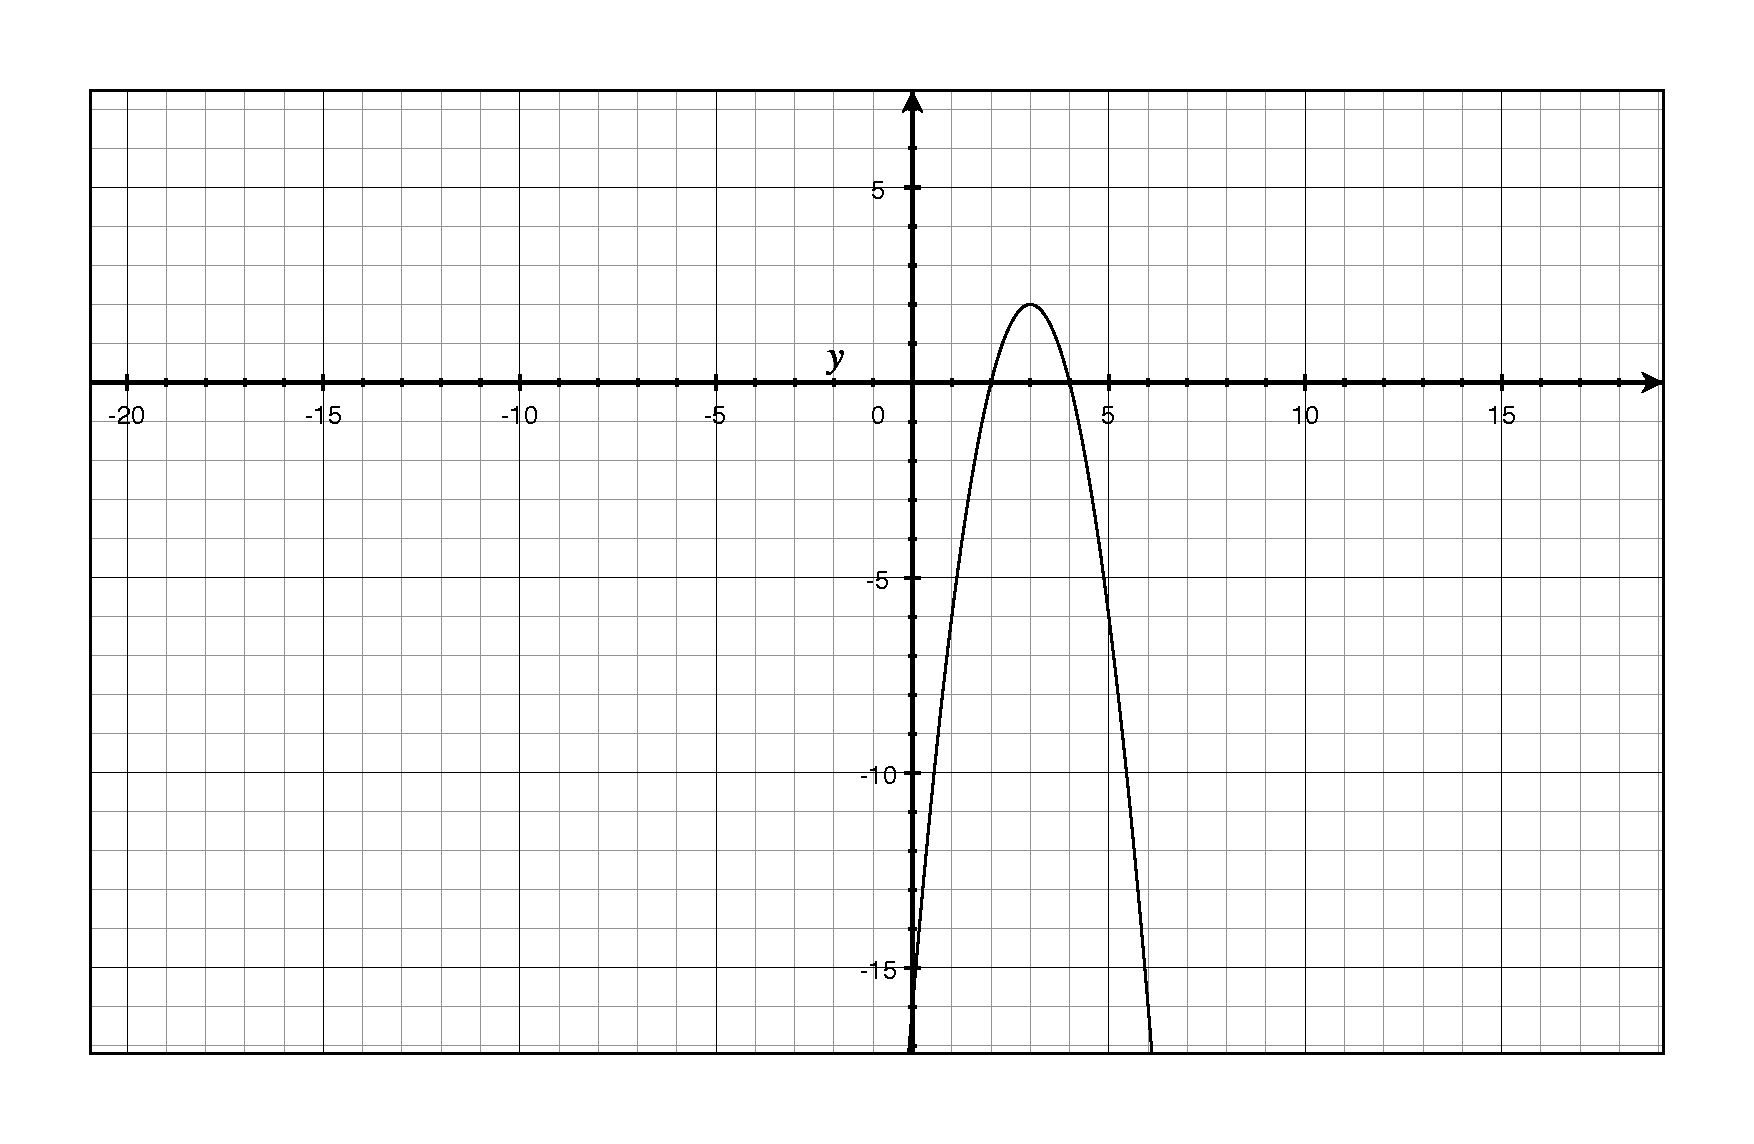
\includegraphics[width=14cm,height=10cm]{prob10.eps}
  \caption*{Problem \ref{quadratic}}
\end{figure}
\else
\begin{figure}[H]
  \centering
  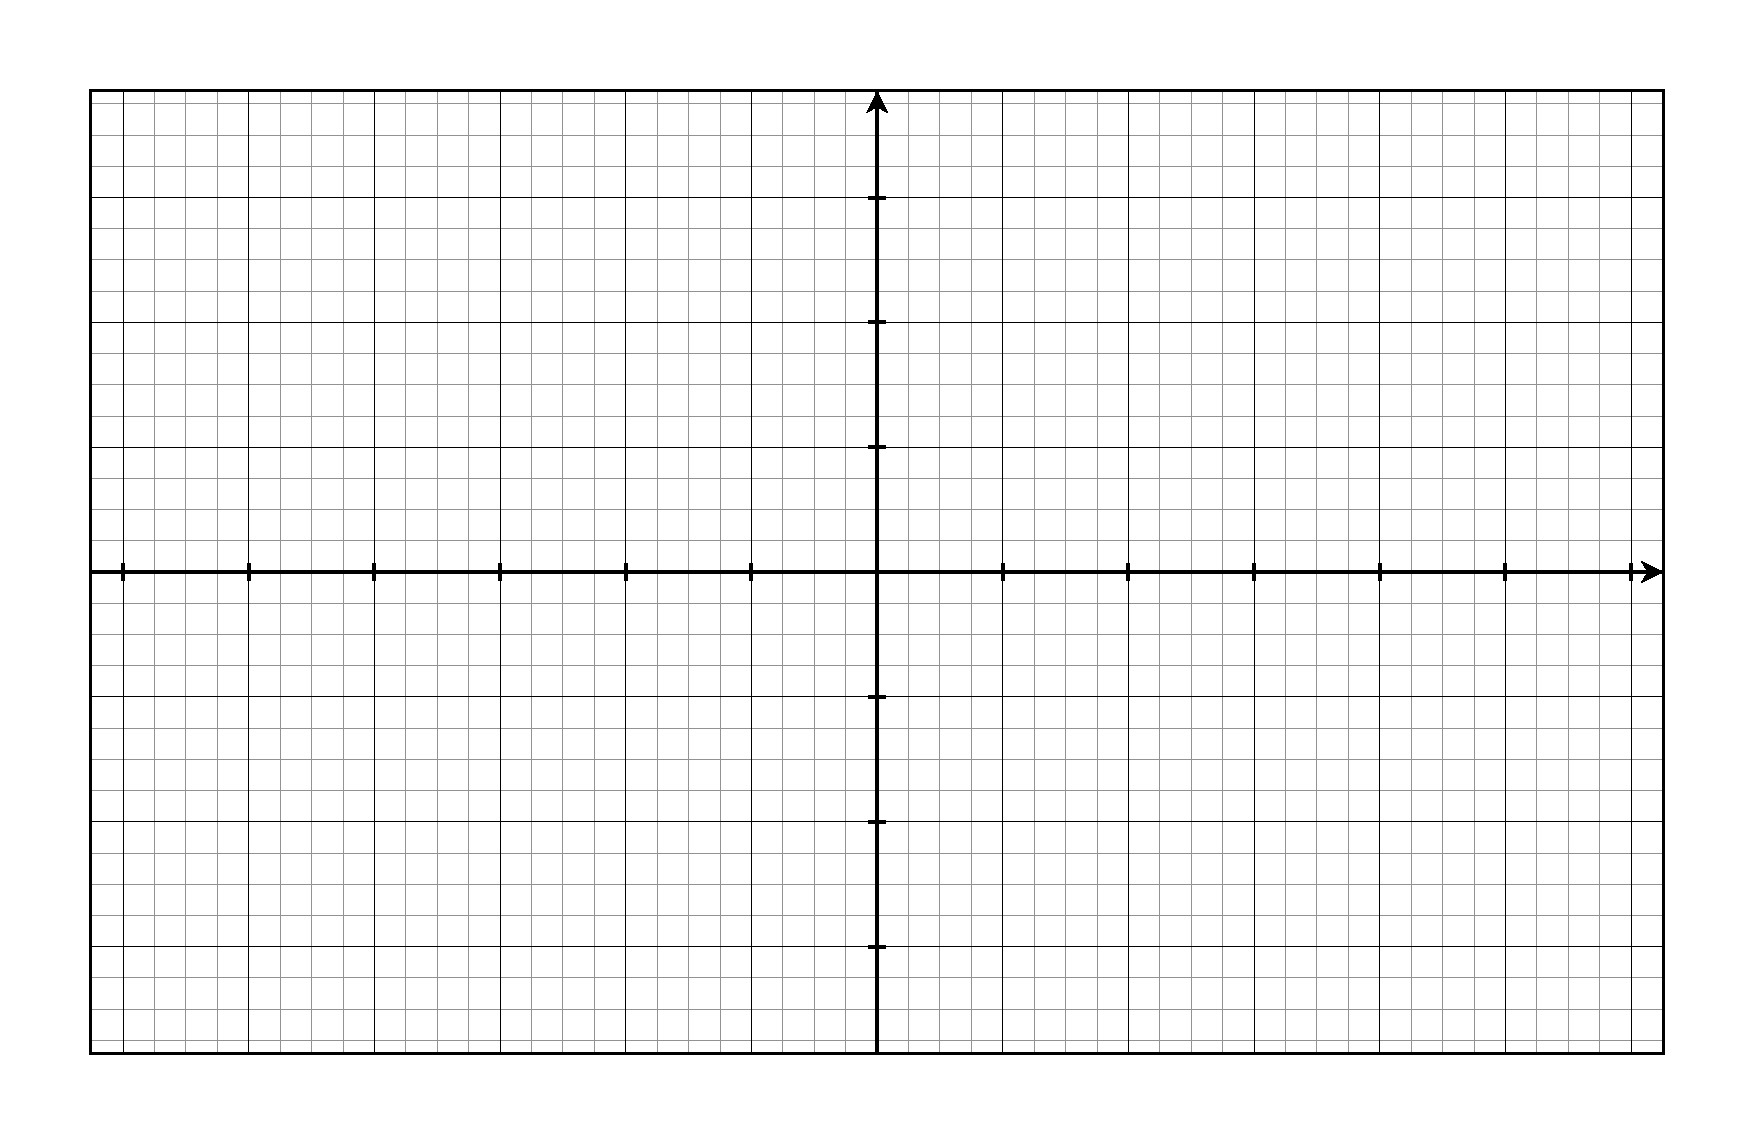
\includegraphics[width=14cm,height=10cm]{quadratic.eps}
  \caption*{Problem \ref{quadratic}}
\end{figure}
\fi

\end{parts}

\ifprintanswers
\pagebreak
\fi

\question
{\em Rupert's Ostrich Feather Coat Factory} has found that the cost to produce $x$ ostrich feather coats in a day is given by the function:
\[
  C(x) = \frac{x^2}{4} - 10x + 800
\]

\begin{parts}
\part[5] How many coats should Rupert produce each day in order to minimize the cost?
\begin{solution}[3 cm]
Since the function is a quadratic, the minimum occurs at the vertex.  The x coordinate of the vertex is at:
\[
    x = \dfrac{-b}{2a} = \dfrac{10}{1/2} = 20
\]
\end{solution}

Rupert should make 20 coats a day to minimize the cost.

\part[2] What is the cost of producing this many coats?
\begin{solution}[2 cm]
\[
  f(20) = \frac{20^2}{4}   - 200 + 800 = 700
\]
\end{solution}

\end{parts}

\pagebreak

\section{Graphing}

\question
\begin{parts}

\part[4] Given the graph of $f(x)$ shown, plot $|f(x)|$ on the same graph
\ifprintanswers
\begin{figure}[H]
  \centering
  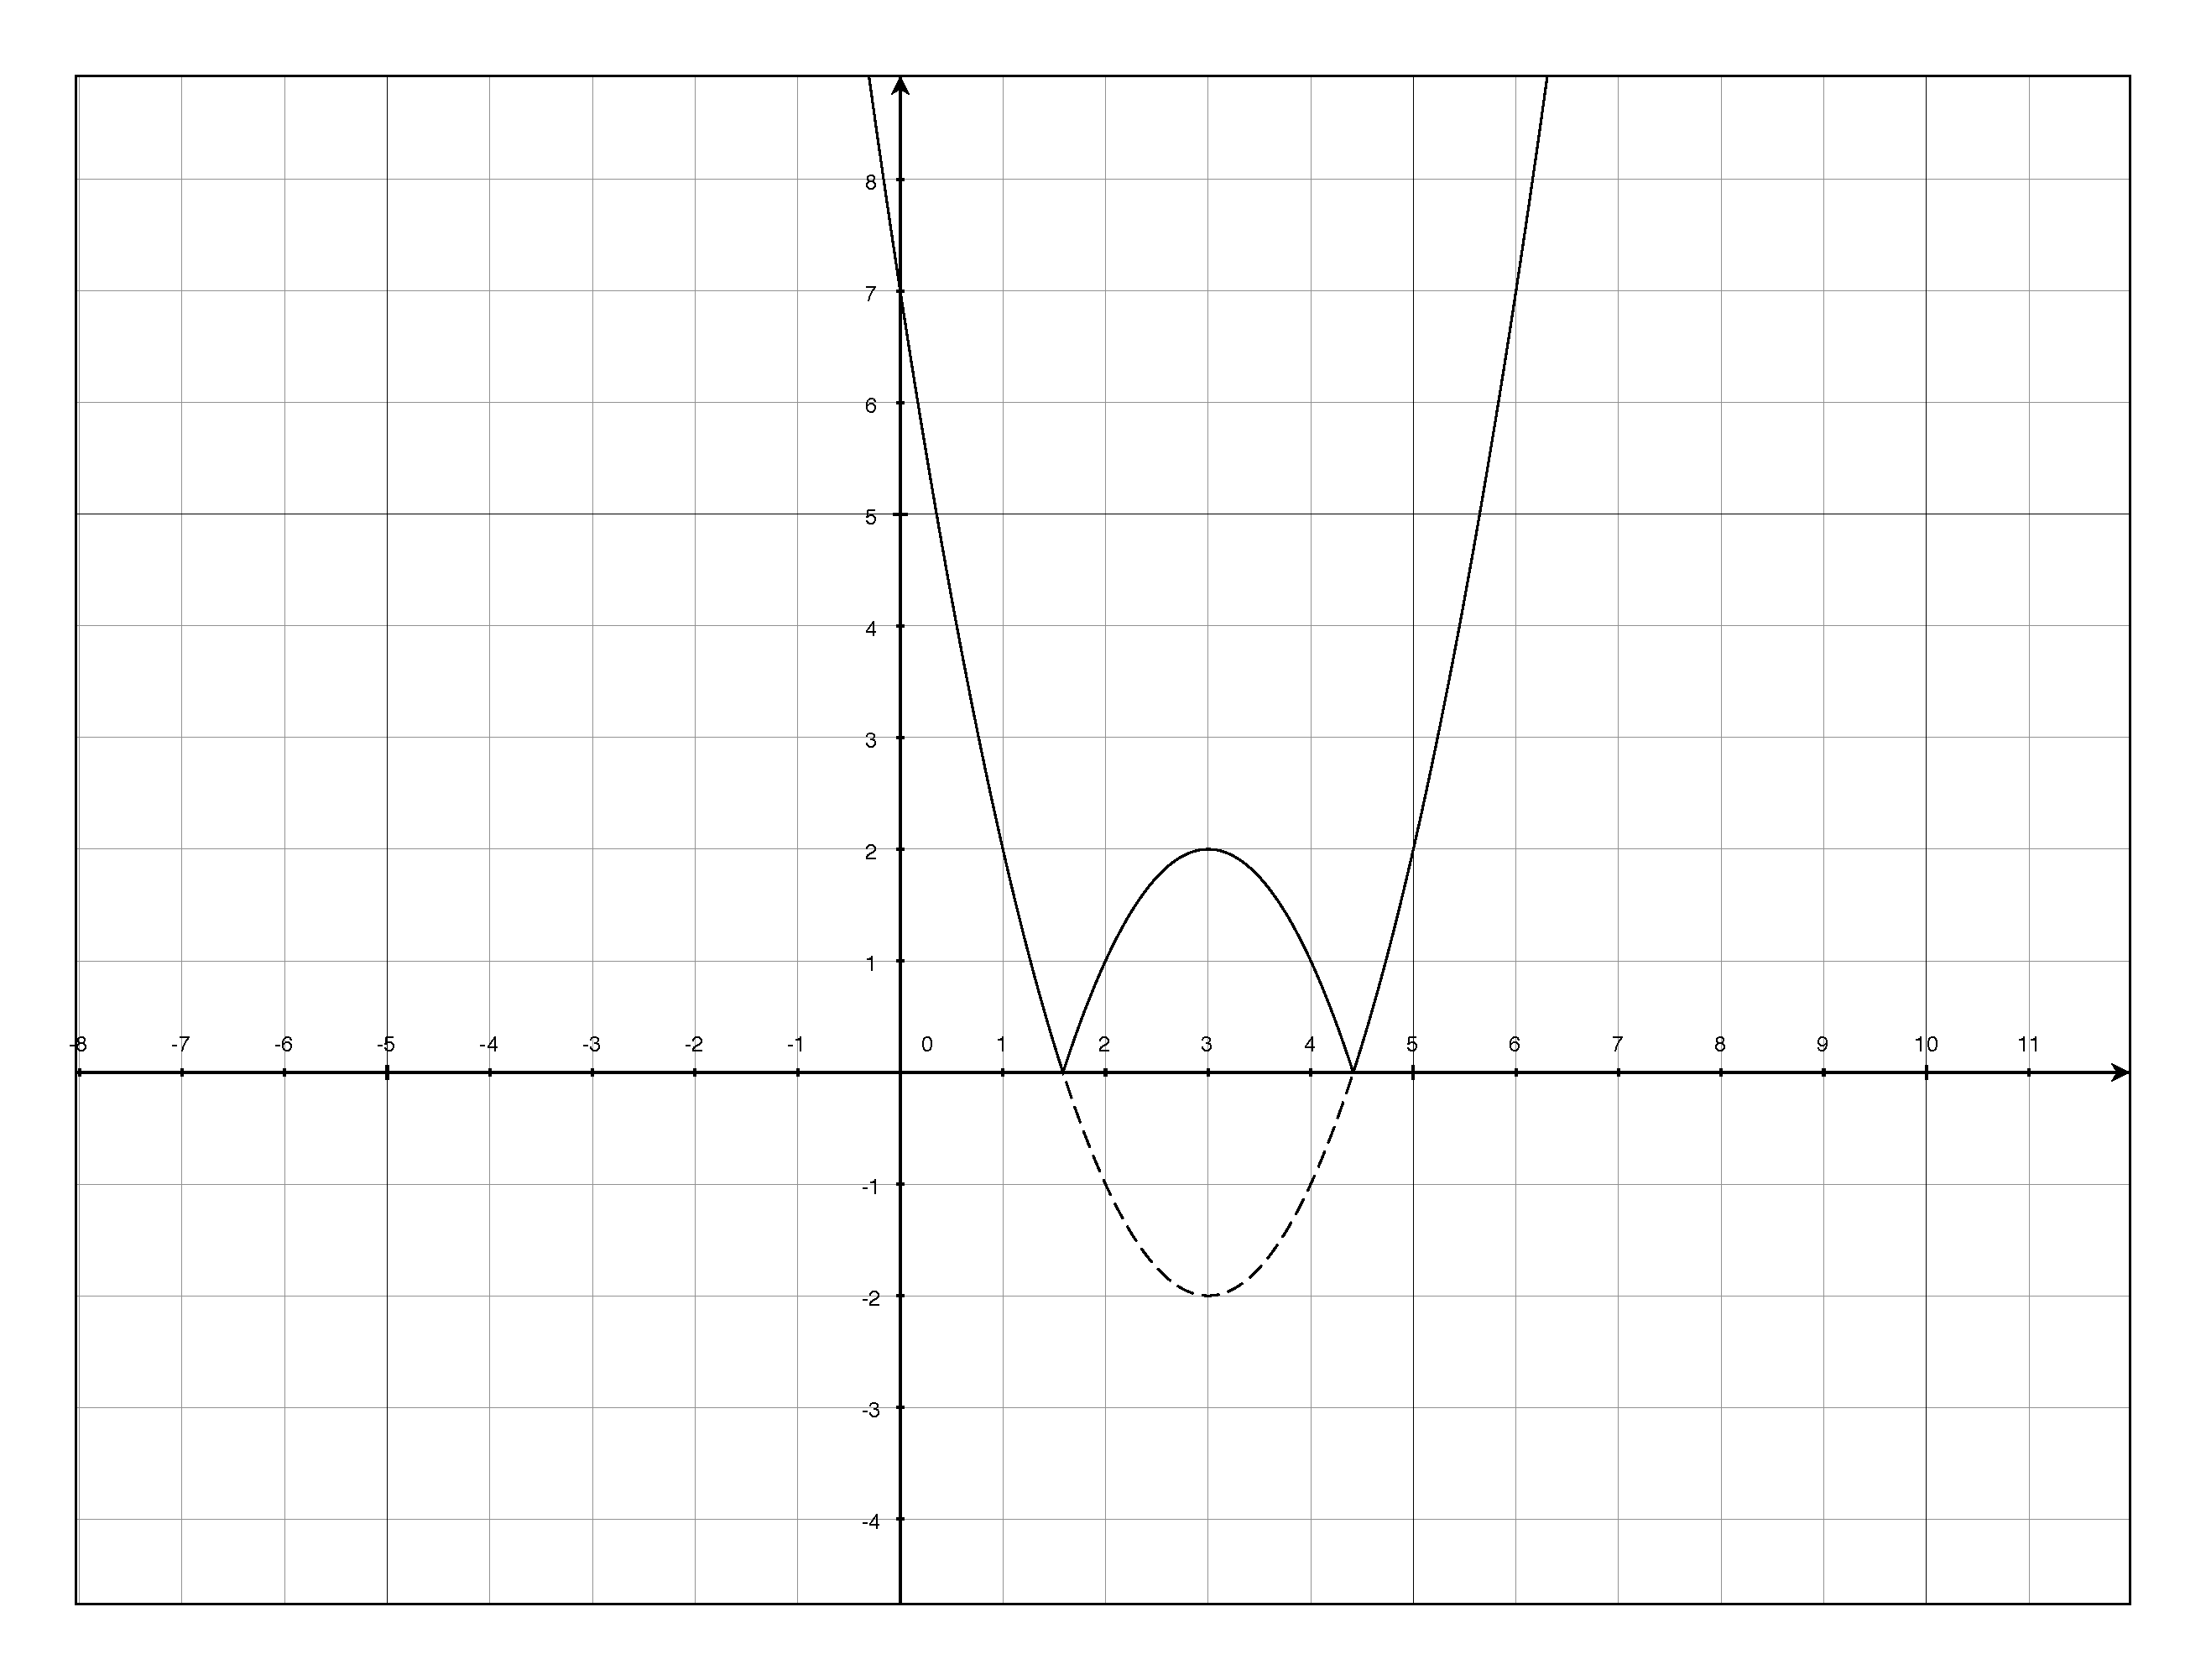
\includegraphics[width=12cm,height=8cm]{prob12a.eps}
  \caption*{$|f(x)|$}
\end{figure}
\else
\begin{figure}[H]
  \centering
  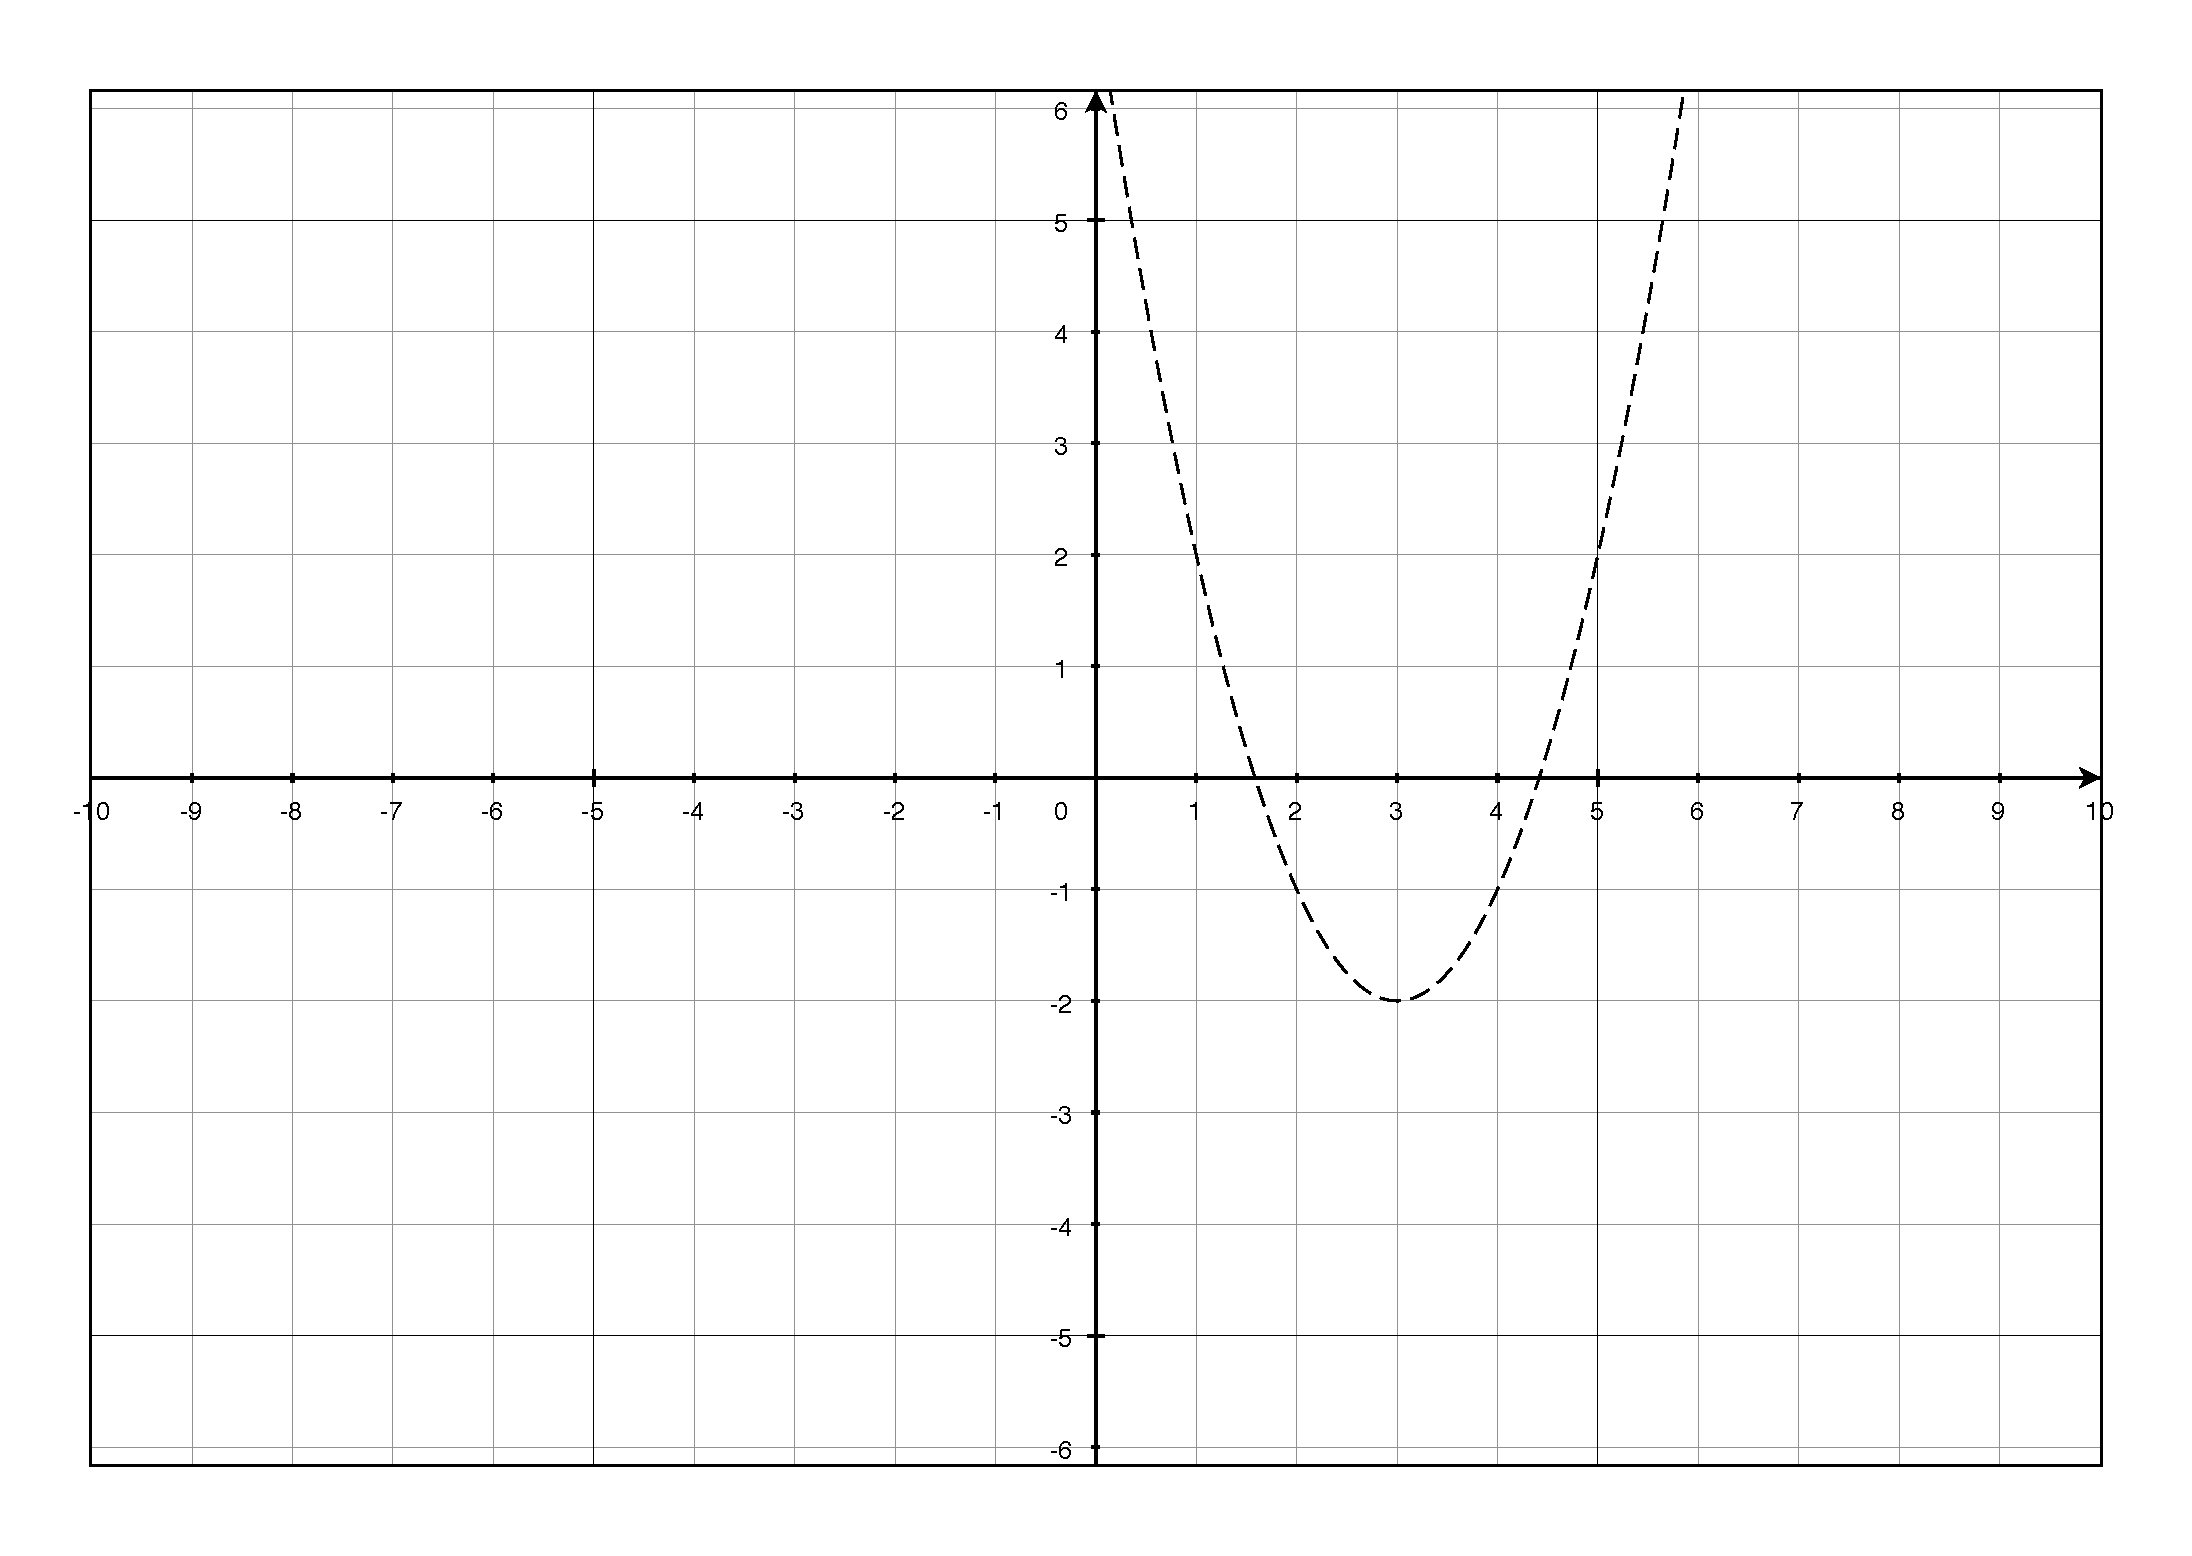
\includegraphics[width=12cm,height=8cm]{graphing.eps}
  \caption*{$|f(x)|$}
\end{figure}
\fi

\ifprintanswers
\pagebreak
\fi

\part[4] Given the graph of $f(x)$ shown, plot $\dfrac{1}{f(x)}$ on the same graph
\ifprintanswers
\begin{figure}[H]
  \centering
  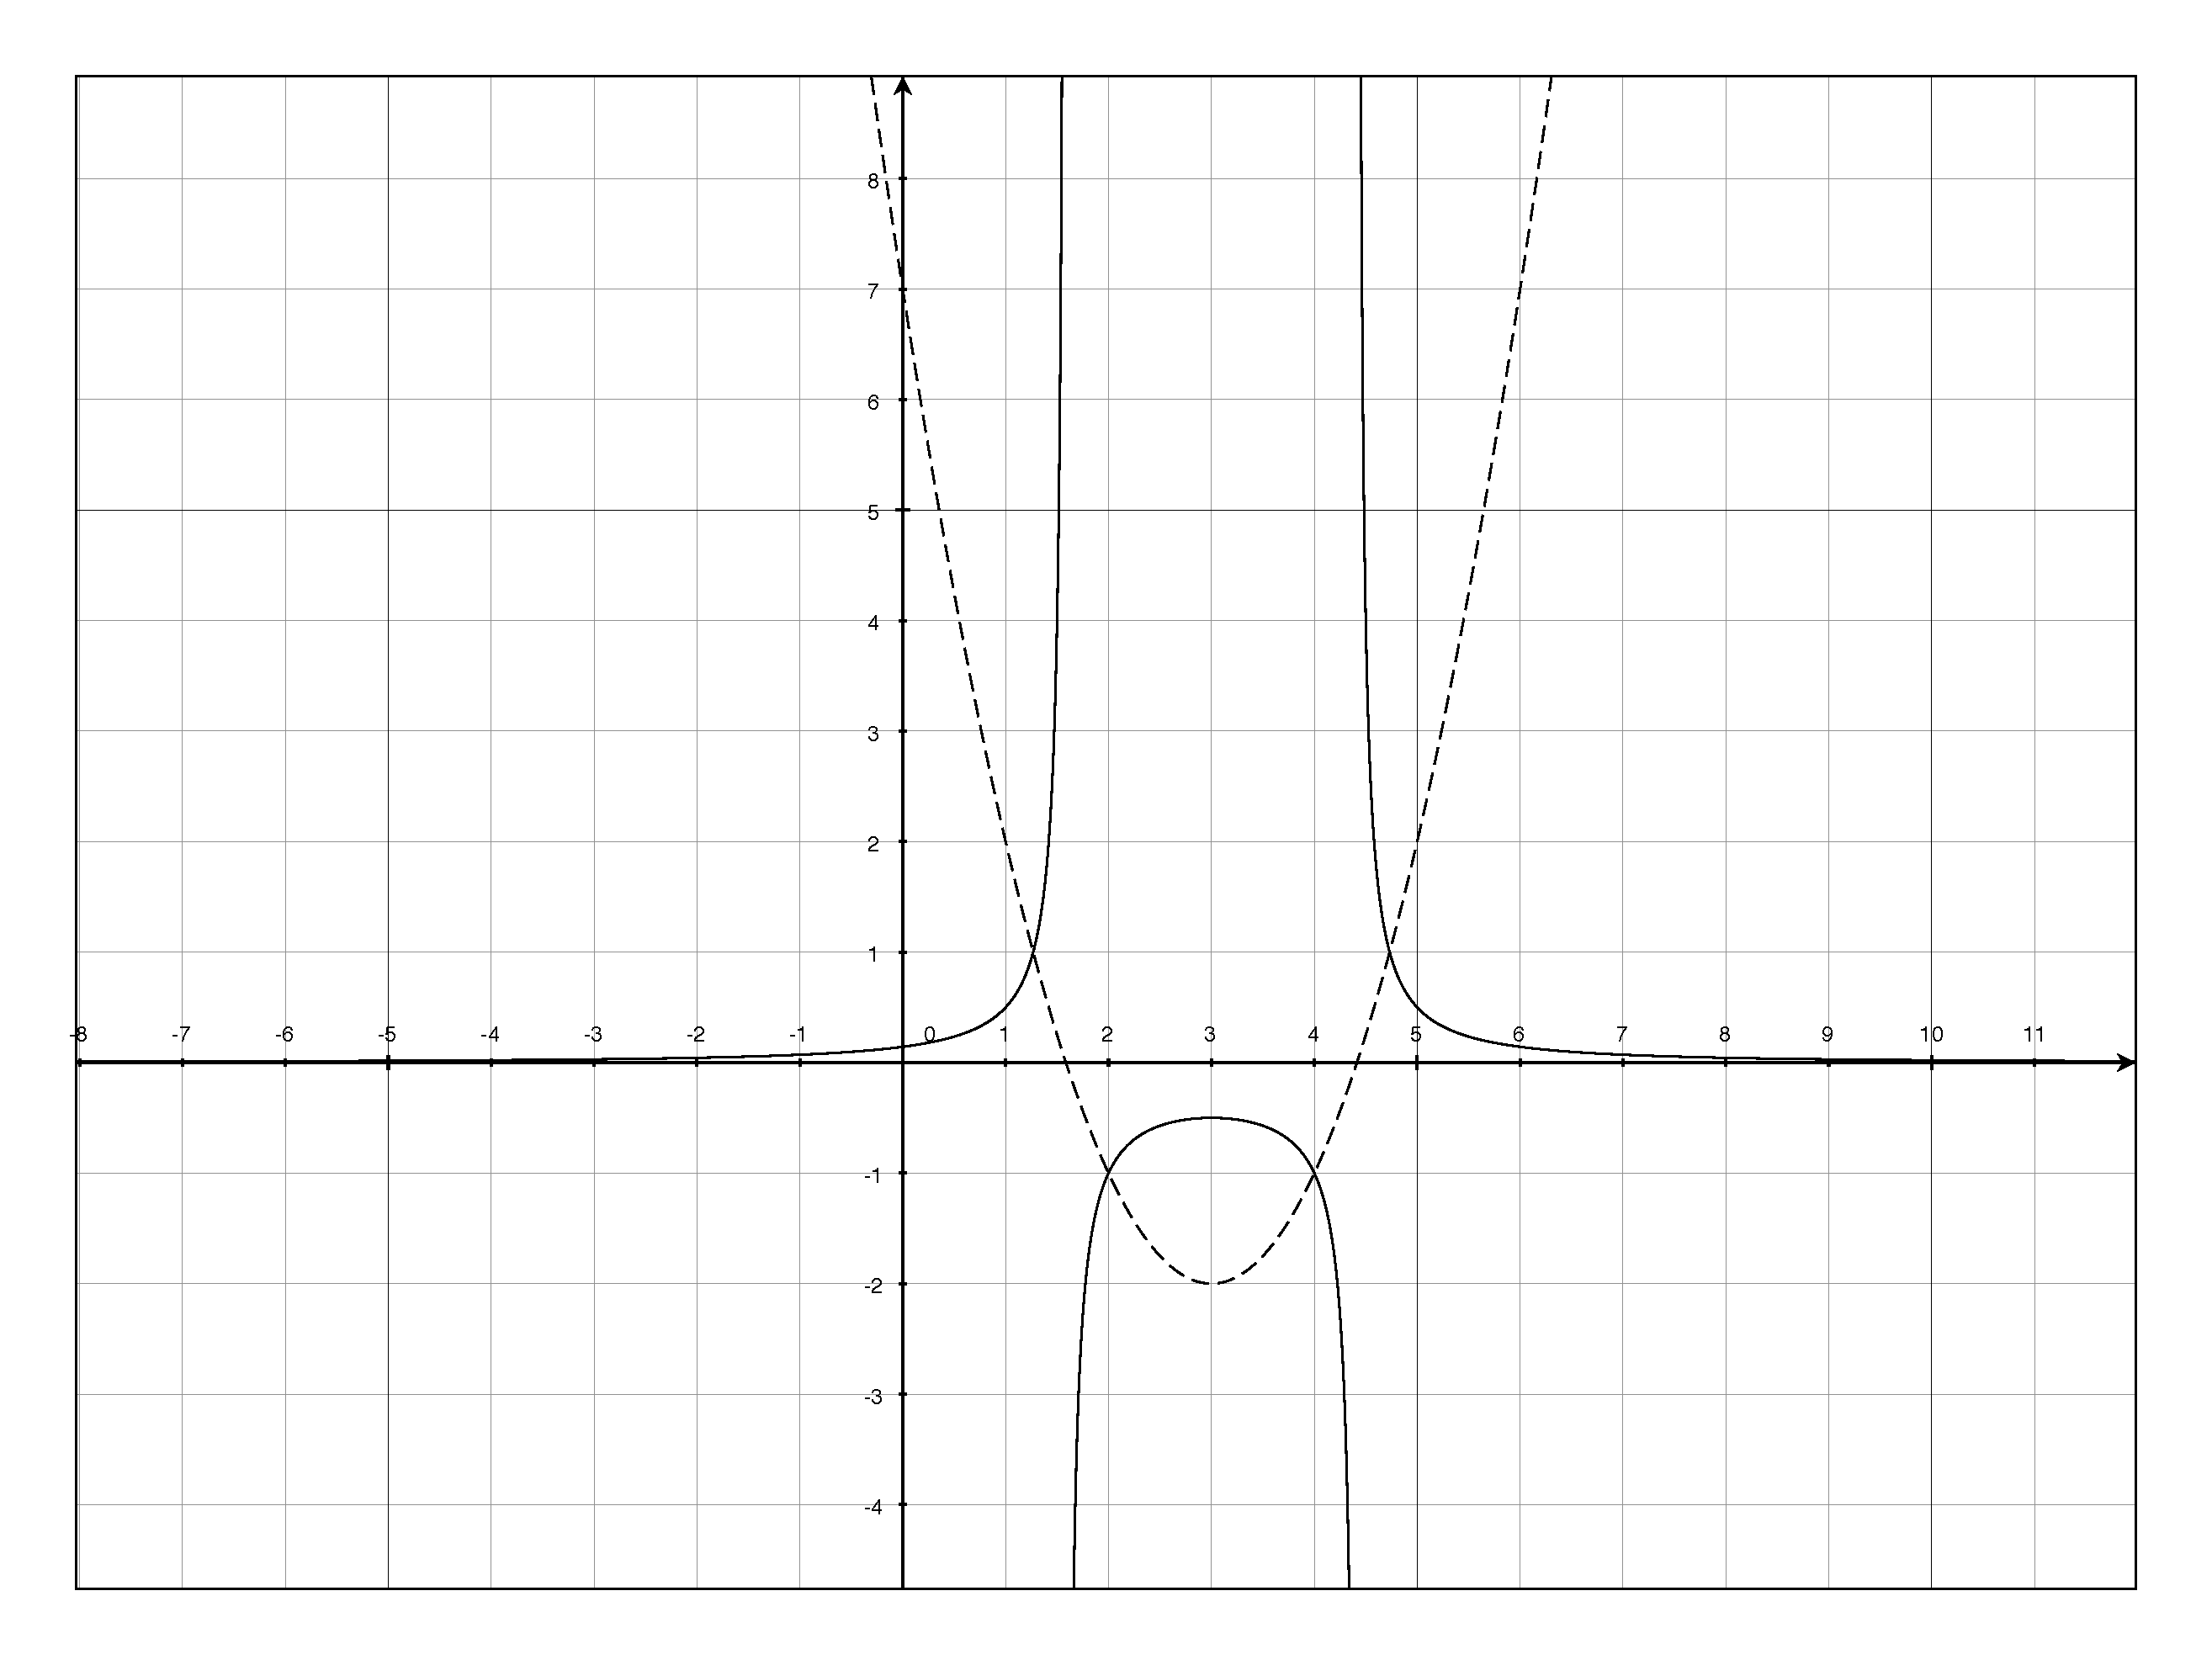
\includegraphics[width=12cm,height=8cm]{prob12b.eps}
  \caption*{$\dfrac{1}{f(x)}$}
\end{figure}
\else
\begin{figure}[H]
  \centering
  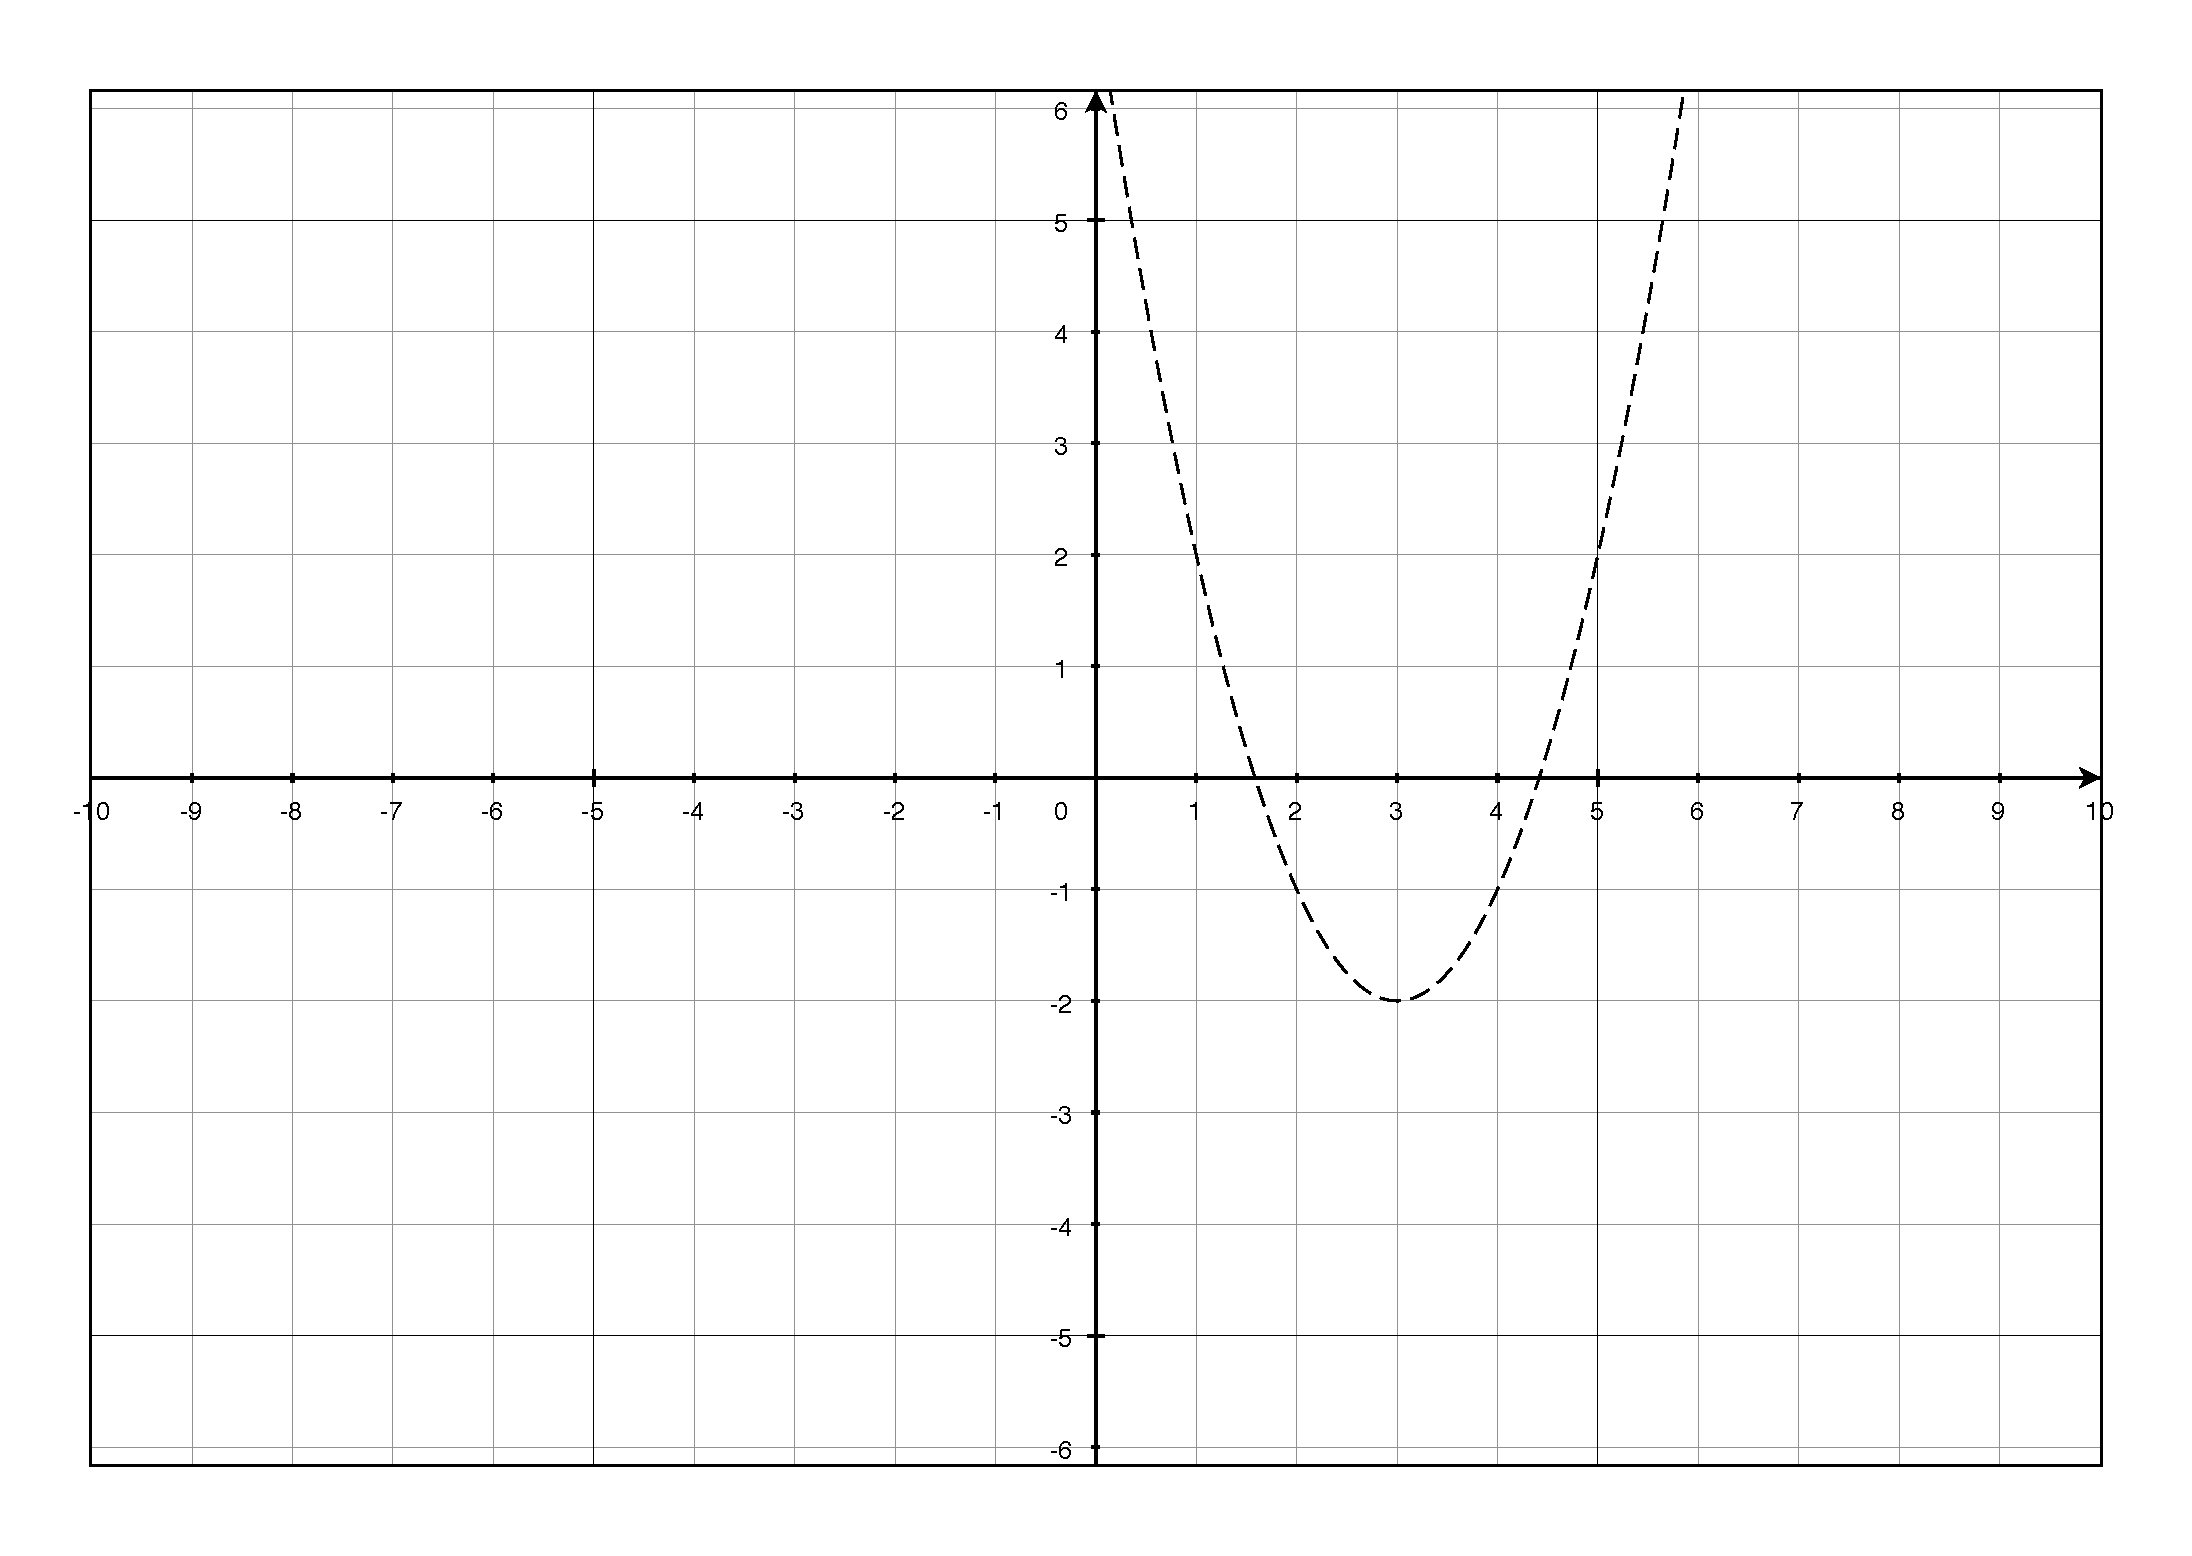
\includegraphics[width=12cm,height=8cm]{graphing.eps}
  \caption*{$\dfrac{1}{f(x)}$}
\end{figure}
\fi

\end{parts}

\section{Extra Credit}
\bonusquestion
This question uses the following formulas for circles:
\begin{itemize}
  \item $C = 2 \pi r$
  \item $A = \pi r^2$
\end{itemize}

Rupert is planning to build a pen for his ostriches.  He doesn't want to spend a lot of money on
fencing, and isn't sure what shape to build the pen in.  He is considering a circle and a square.

\begin{parts}

\bonuspart[2] Find a function $s(p)$ which gives the length of the sides of a square with perimeter $p$.
\begin{solution}[2 cm]
\[
  s(p) = \frac{p}{4}  
\]
\end{solution}

\bonuspart[3] Find a function $A_{square}(p)$ which gives the area of a square with perimeter $p$.
\begin{solution}[3 cm]
The function for the area of a square in terms of the sides is: $A(s) = s^2$.
\[
  A_{square}(p) = A \circ s = \left( \frac{p}{4} \right)^2 = \frac{p^2}{16}
\]
\end{solution}

\bonuspart[2] Find a function $r(c)$ which gives the length of the radius of a circle with circumference $c$.
\begin{solution}[3 cm]
\[
  r(c) = \frac{c}{2 \pi}  
\]
\end{solution}

\bonuspart[3] Find a function $A_{circle}(c)$ which gives the area of a circle with circumference $c$.
\begin{solution}[3 cm]
\[
    A_{circle}(c) = A \circ r = \pi \left( \frac{c}{2 \pi} \right)^2 = \frac{c^2}{4 \pi}
\]
\end{solution}

\bonuspart[5] \label{ostrich:best} Which shape should he build and why?
\begin{solution}[2 cm]
Since $4 \pi < 16$, $\dfrac{x^2}{4 \pi} > \dfrac{x^2}{16}$ and the circular pen is the better choice.
\end{solution}

% \bonuspart[5] Rupert is going to the fencing store to pick up some fencing materials.  He knows that each ostrich needs 10 square
% meters of space to roam about in.  Using your answer to part \ref{ostrich:best}, find a function $f(n)$ which provides the
% length of fencing needed to hold $n$ ostriches.
% \begin{solution}[4 cm]
% \end{solution}

\end{parts}


\end{questions}

\end{document}
